\begin{frame}[label=intro]{Introduction}
    
    \begin{exampleblock}{What?}
        Cryptanalysis of the \textbf{Permuted Congruential Generator} (PCG).
    \end{exampleblock}
    
    \medskip
    
    \begin{alertblock}{Results}
      \textbf{Practical seed-recovery} / prediction.
    \end{alertblock}
    
    \begin{block}{How?}
    \begin{itemize}
        \item "Guess-and-Determine" attack.
        \item Most expensive part : many small CVP problems.
        \item \textbf{Actually done} in $\leq$ 20 000 CPU-hours.
    \end{itemize}  
    \end{block}
\end{frame}

\begin{frame}{Why?}
    \centering
    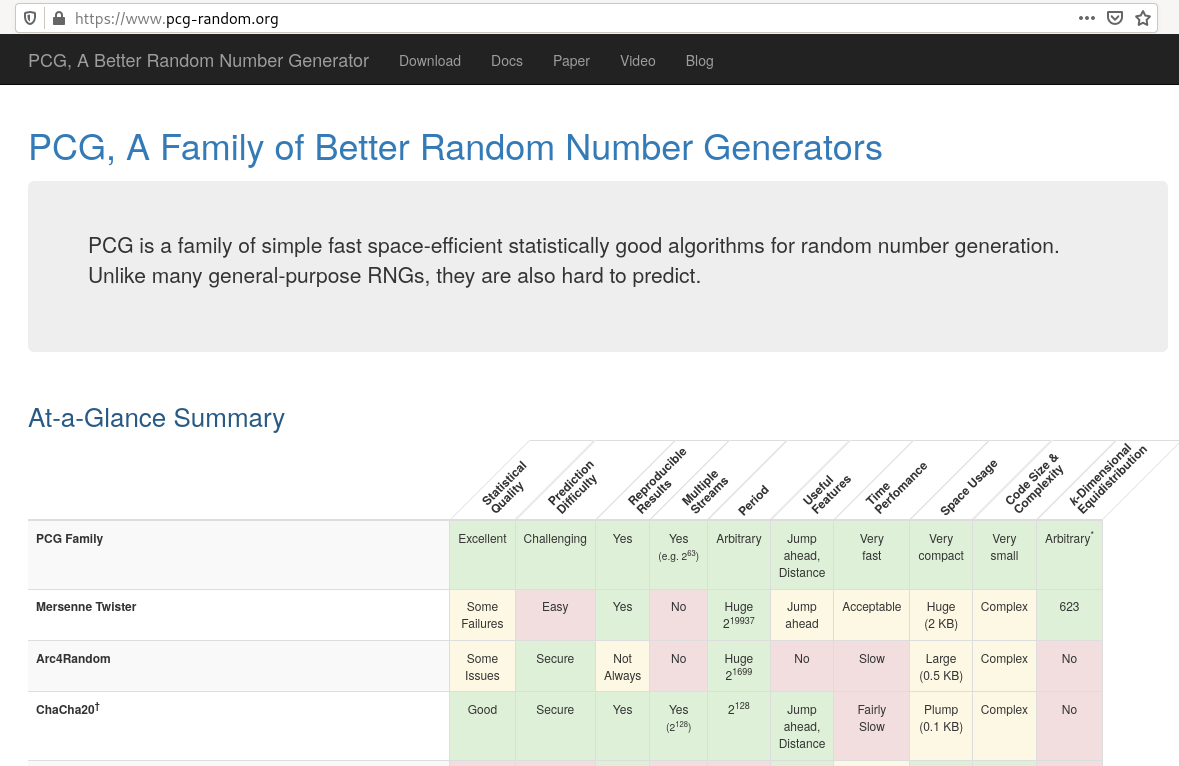
\includegraphics[width=\textwidth]{pictures/website.png}
\end{frame}

\begin{frame}{Why?}
    \centering
    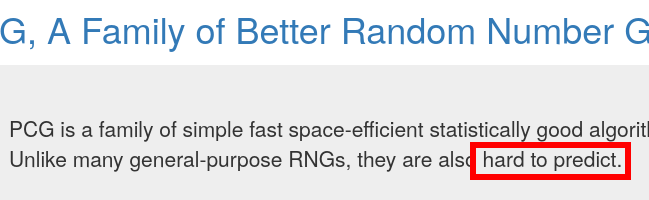
\includegraphics[width=\textwidth]{pictures/hard.png}
\end{frame}

\begin{frame}{Why?}
    \centering
    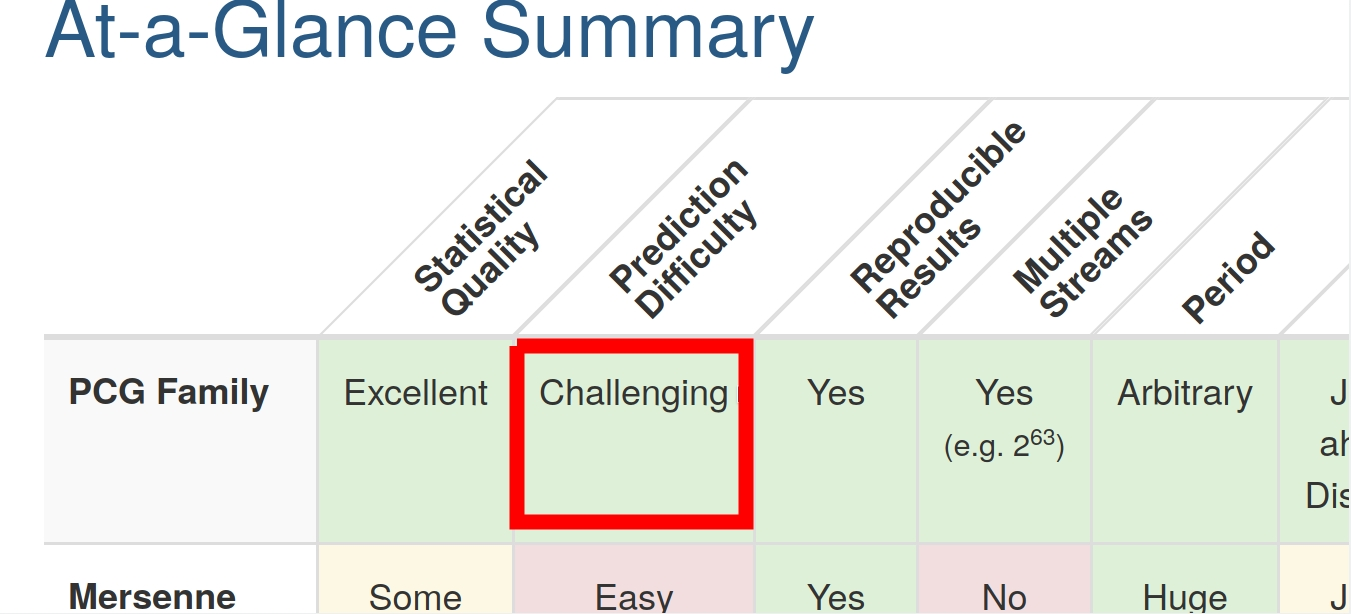
\includegraphics[width=0.9\linewidth]{pictures/PCG_challenging.jpg}
\end{frame}

\begin{frame}
    \centering
    
\includegraphics[height=\textheight]{pictures/accepted.jpg}
\end{frame}

\againframe{intro}

\begin{frame}{Permuted Congruencial Generators (\textsf{PCG})}
    \begin{itemize}
        \item Conventional (non-crypto) pseudo-random generators
        \item Designed in 2014 by Melissa O'Neil
        \item Version studied : \textsf{PCG64}
        \begin{itemize}
            \item Internal state : 128-bit state and 128-bit \alert{increment}
            \item 64-bit outputs
            \item 256-bit seed (or 128-bit with default increment)
            \item Default pseudo-random generator in \textsf{NumPy}
        \end{itemize}
    \end{itemize}

    \begin{center}
    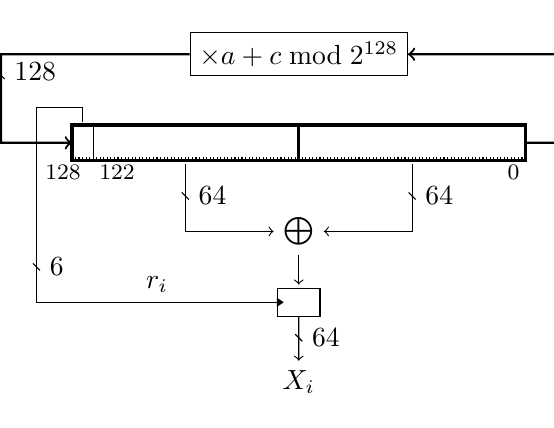
\begin{tikzpicture}[scale=0.45]
      \path[red, use as bounding box] (-1.25, -6.75) rectangle (12.8, 3.75);
      
      % S_i
    
        % bordures
        \draw[very thick]  (0, 0) rectangle (12.8, 1);
        \draw<4->  (0.6, 0) rectangle +(0, 1);
        \draw<3->[very thick]  (6.4, 0) rectangle +(0, 1);
        \foreach \i in {0, 1, ..., 128} \draw (\i/10, 0) -- +(0, 0.1);
        
        % déco autour
        \node<2->[draw] at (6.4, 3) (update) {$\times a + \alert{c} \bmod 2^{128}$};
        \draw<2->[thick,->] (12.8, 0.5) -- (13.8, 0.5) node[below right] {$S_i$} -- (13.8, 3) -- (update);
        \draw<2-> (13.7, 2.5) -- +(0.2, -0.2);
        \path<2-> (13.9, 2.5) node[anchor=west] {128};
        \draw<2->[thick,->] (update) -- (-2, 3) -- (-2, 0.5) node[below left] {$S_{i+1}$} -- (0, 0.5);
        \draw<2-> (-2.1, 2.5) -- +(0.2, -0.2);
        \path<2-> (-1.9, 2.5) node[anchor=west] {128};
    
        
        \node[font=\footnotesize,anchor=east] at (12.9, -0.33) {0};
        %\node<3->[font=\footnotesize,anchor=east] at (6.5, -0.33) {64};
        \node<4->[font=\footnotesize,anchor=west] at (0.5, -0.33) {122};
        \node[font=\footnotesize] at (-0.25, -0.33) {128};
        
        \draw<3-> (6.4, -2) node (x) {$\bigoplus$};
        
        \draw<3->[->] (3.2, -0.1) |- (x);
        \draw<3-> (3.1, -0.9) -- +(0.2, -0.2);
        \path<3-> (3.3, -1) node[anchor=west] {64};
        
        \draw<3->[->] (9.6, -0.1) |- (x);
        \draw<3-> (9.5, -0.9) -- +(0.2, -0.2);
        \path<3-> (9.7, -1) node[anchor=west] {64};
    
        \node<4>[minimum width=1.8cm] at (6.4, -4) (r) {$\ggg$};
        \draw<4> (5.8, -3.6) rectangle +(1.2, -0.8);
        \draw<4>[fill=black] (5.8, -4.1) -- (5.95, -4) -- (5.8, -3.9) -- cycle;
        
        \draw<4> (0.3, 1.1) -- (0.3, 1.5) -- (-1, 1.5) -- (-1, -4) -- node[above] {$r_i$} (5.8, -4);
        \draw<4> (-1.1, -2.9) -- +(0.2, -0.2);
        \path<4> (-0.9, -3) node[anchor=west] {6};
    
        \draw<3->[->] (x) -- +(0, -1.5);
        \node<4> at (6.4, -6.25) (xi) {$X_i$};
        \draw<4>[->] (6.4, -4.4) -- (xi);
    
        \draw<4> (6.3, -4.9) -- +(0.2, -0.2);
        \path<4> (6.5, -5) node[anchor=west] {64};
      \end{tikzpicture}
    \end{center}

  \end{frame}


%%% Local Variables:
%%% mode: latex
%%% TeX-master: "../main"
%%% End:
